\documentclass[11pt,a4paper]{article}

\usepackage[margin=1in]{geometry}
\usepackage{titlesec}
\usepackage{enumitem}
\usepackage{hyperref}
\usepackage{parskip}
\usepackage{graphicx}
\usepackage{float}
\usepackage{booktabs}
\usepackage{amsmath}

\hypersetup{colorlinks=true, linkcolor=blue, urlcolor=blue}

\titleformat{\section}{\large\bfseries}{\thesection}{0.5em}{}
\titleformat{\subsection}{\normalsize\bfseries}{\thesubsection}{0.5em}{}
\setlist{leftmargin=1.4em, topsep=2pt, itemsep=2pt}

\title{\vspace{-1.5cm}\textbf{PKCERT AI \& Software Development Internship \\ Task 19: Training Loops -- Loss Functions, Optimizers, Epoch/Batch Management}}
\author{Abdullah Amir}
\date{AI and Software Development \\ 29 July 2026}

\begin{document}

\maketitle
\vspace{-0.8cm}

This report covers the theory, derivations and results. The full code and outputs live
in the notebook \texttt{training\_loops.ipynb}. \textbf{PyTorch 2.13.0 (CPU build)} is
used throughout. Task 18 called \texttt{torch.optim} as a black box; this task opens it:
SGD, SGD+momentum and Adam are implemented as manual parameter-update loops and verified
step-for-step against \texttt{torch.optim} on a toy convex function, and every major
training-loop mechanism is demonstrated on a case constructed specifically to exercise
it, with a fixed random seed (42) throughout for reproducibility.

% ----------------------------------------------------------------
\section*{Part A: Loss Functions in Depth}

\textbf{Four losses from scratch}, verified against PyTorch's built-ins to within
$10^{-6}$: MSE, L1, cross-entropy (log-sum-exp with max-subtraction for stability, built
by hand rather than called) and binary hinge loss. All four matched their references to
floating-point precision.

\textbf{Cross-entropy vs MSE, made numerically concrete.} Backpropagated through
softmax, cross-entropy's gradient simplifies to the clean $dL/dz = p - y$ on the
pre-softmax logits, which does not vanish just because $p$ is near 0 or 1. MSE computed
directly on softmax probabilities picks up an extra factor of $p(1-p)$ -- the softmax's
own derivative -- which collapses toward 0 exactly as $p$ saturates. On a constructed
confidently-wrong prediction ($p=0.0003$ for the true class), the measured gradients
were cross-entropy $\approx 0.9997$ versus MSE-on-softmax $\approx 0.000447$ --
\textbf{cross-entropy's gradient was $\sim$2239x larger}, precisely on the case that
most needs a large correction.

\textbf{L2-regularised custom loss, hand-derived and checked against autograd.}
\[
L(w) = \text{MSE}(Xw, y) + \frac{\lambda}{2}\|w\|^2 \qquad
\frac{dL}{dw} = \frac{2}{N}X^\top(Xw - y) + \lambda w
\]
Maximum absolute difference between this hand-derived gradient and autograd's:
$1.19\times10^{-7}$ -- a match.

\textbf{Class imbalance and a from-scratch weighted cross-entropy.} On a 90:10
synthetic imbalance, unweighted cross-entropy's total gradient contribution split
exactly 9.0:1 between majority and minority classes -- matching the sample ratio
precisely, meaning the rare class's gradient signal is diluted in direct proportion to
how rare it is. Inverse-frequency class weighting ($w_c = N / (\text{n\_classes} \cdot
n_c)$) rebalanced this to a measured 1.00:1 ratio, restoring the two classes' equal pull
on the parameters regardless of how many samples of each appear in a given batch.

% ----------------------------------------------------------------
\section*{Part B: Optimizers -- SGD and Adam Internals}

\textbf{Toy function}: $f(x,y) = x^2 + 10y^2$, an elongated bowl from $(5,5)$, so
momentum and Adam have a genuine reason to diverge from vanilla SGD's behaviour.

\begin{table}[H]
\centering
\begin{tabular}{lr}
\toprule
\textbf{Optimizer} & \textbf{Max trajectory diff, manual vs torch.optim (40 steps)} \\
\midrule
Vanilla SGD & $2.4\times10^{-7}$ \\
SGD + momentum (0.9) & $4.8\times10^{-7}$ \\
Adam (default $\beta_1,\beta_2,\epsilon$) & $4.8\times10^{-7}$ \\
\bottomrule
\end{tabular}
\caption{All three from-scratch optimizers match torch.optim step-for-step.}
\end{table}

\begin{figure}[H]
    \centering
    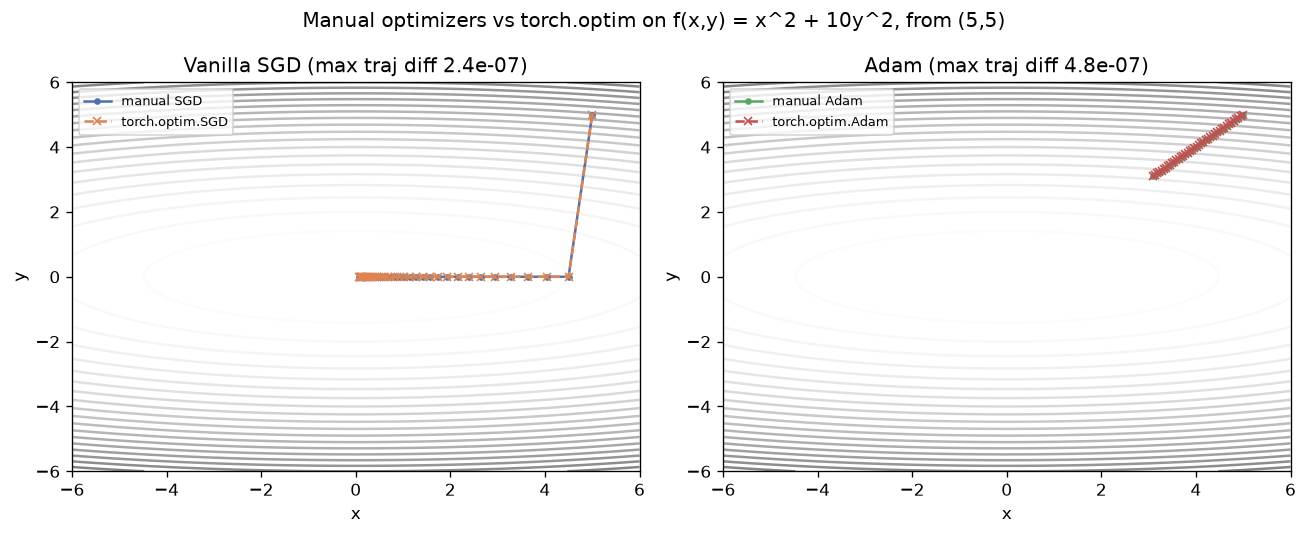
\includegraphics[width=0.95\textwidth]{figures/01_optimizer_verification.png}
    \caption{Manual SGD and Adam trajectories overlaid exactly on their torch.optim counterparts.}
\end{figure}

The residual $\sim10^{-7}$ differences are consistent with PyTorch's default epsilon
placement \emph{outside} the square root ($lr \cdot \hat{m} / (\sqrt{\hat{v}} +
\epsilon)$, the formula matched here, following the original Adam paper); a variant
placing $\epsilon$ inside the square root would diverge slightly more, especially while
$\hat v$ is still small in the first few steps.

\textbf{Worked example: Adam on unevenly-scaled gradients.} For
$f(x,y) = x^2 + 1000y^2$, $\nabla f = (2x, 2000y)$ -- the $y$-gradient is 1000x the
$x$-gradient at equal distance from the minimum. SGD at the largest stable step for $y$
made only 0.045 of progress on $x$ in 5 steps, forced to crawl at the pace of the
worst-scaled dimension. Adam, dividing each parameter's update by its own running RMS
gradient, made \textbf{comparable progress on both axes} (2.46 on $x$, 2.46 on $y$)
despite the 1000x scale gap -- the adaptive denominator cancels exactly the scale
difference between dimensions.

\subsection*{Controlled 3-way comparison: SGD, SGD+momentum, Adam}

Same network (the Palmer Penguins $4\to8\to3$ net from Task 17/18), same
initialisation, same data.

\begin{table}[H]
\centering
\begin{tabular}{lrr}
\toprule
\textbf{Optimizer} & \textbf{Final training loss} & \textbf{Validation accuracy} \\
\midrule
SGD (lr=0.1) & 0.0934 & 0.9855 \\
SGD+momentum (lr=0.1, m=0.9) & \textbf{0.0123} & \textbf{1.0000} \\
Adam (lr=0.01) & 0.0330 & \textbf{1.0000} \\
\bottomrule
\end{tabular}
\end{table}

\begin{figure}[H]
    \centering
    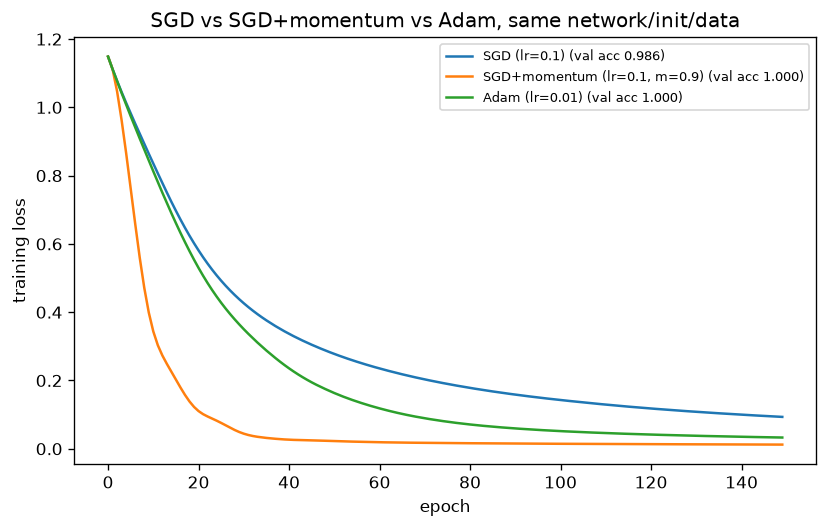
\includegraphics[width=0.68\textwidth]{figures/02_optimizer_comparison_penguins.png}
    \caption{SGD+momentum reaches the lowest loss and the fastest, smoothest descent of the three.}
\end{figure}

\textbf{Tuned SGD+momentum beat Adam}, a result returned to in Part D: Adam's adaptive
scaling is built for exactly the pathology demonstrated above (wildly uneven gradient
scales); this small, well-conditioned network has none of that, so Adam's extra
machinery buys nothing here.

\subsection*{L2-in-gradient vs AdamW's decoupled weight decay}

\begin{table}[H]
\centering
\begin{tabular}{llr}
\toprule
\textbf{Optimizer} & \textbf{Comparison} & \textbf{Max abs.\ difference} \\
\midrule
SGD & L2-in-gradient vs decoupled decay & $1.2\times10^{-7}$ (equivalent) \\
Adam & L2-in-gradient vs AdamW (decoupled) & $0.0668$ (NOT equivalent) \\
\bottomrule
\end{tabular}
\caption{Same toy 2-parameter example, deliberately uneven gradient scales (10 vs 0.1).}
\end{table}

For plain SGD, adding $\lambda w$ to the gradient and shrinking $w$ by
$(1-lr\cdot\lambda)$ after the step are the same arithmetic -- confirmed to
floating-point precision. For Adam, feeding the L2 term into the gradient means it also
gets folded into $v$ (the squared-gradient running average) and divided by
$\sqrt{\hat v}$ along with the data gradient, so the same nominal decay is scaled
\emph{down} for the large-gradient parameter and, relatively, \emph{up} for the
small-gradient one. AdamW's decoupled decay applies the same shrinkage to every
parameter regardless of its gradient history -- the behaviour weight decay is actually
supposed to have, and measurably different (0.0668) from L2-in-the-gradient here.

% ----------------------------------------------------------------
\section*{Part C: Epochs, Batches, and Training Loop Engineering}

\textbf{Batch GD vs mini-batch GD vs SGD}, same data/model/learning rate (0.05, 60
epochs). Batch GD (1 update/epoch) reached 0.431; mini-batch (B=32, 9 updates/epoch)
reached 0.050; single-sample SGD (273 updates/epoch) reached 0.012 -- more, noisier
updates per epoch converged faster at this fixed learning rate.

\begin{figure}[H]
    \centering
    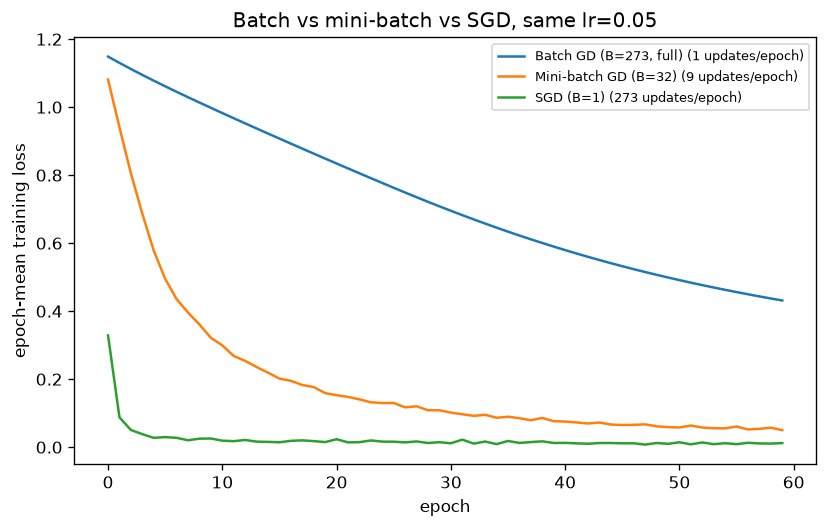
\includegraphics[width=0.68\textwidth]{figures/03_batch_vs_minibatch_vs_sgd.png}
    \caption{Batch GD, mini-batch GD and SGD, same LR: more updates/epoch, faster descent.}
\end{figure}

\subsection*{Batch size sweep}

\begin{table}[H]
\centering
\begin{tabular}{lrrrr}
\toprule
\textbf{Batch size} & \textbf{Wall-clock (80 ep.)} & \textbf{Epochs to loss$<$0.3} & \textbf{Val acc} & \textbf{Train$-$val gap} \\
\midrule
8   & 0.660s & 4  & 1.0000 & \textbf{0.0000} \\
32  & 0.414s & 11 & \textbf{1.0000} & $-$0.0110 \\
128 & 0.221s & 29 & 0.9855 & $-$0.0148 \\
273 (full) & \textbf{0.159s} & never & 0.8696 & $+$0.0535 \\
\bottomrule
\end{tabular}
\end{table}

\begin{figure}[H]
    \centering
    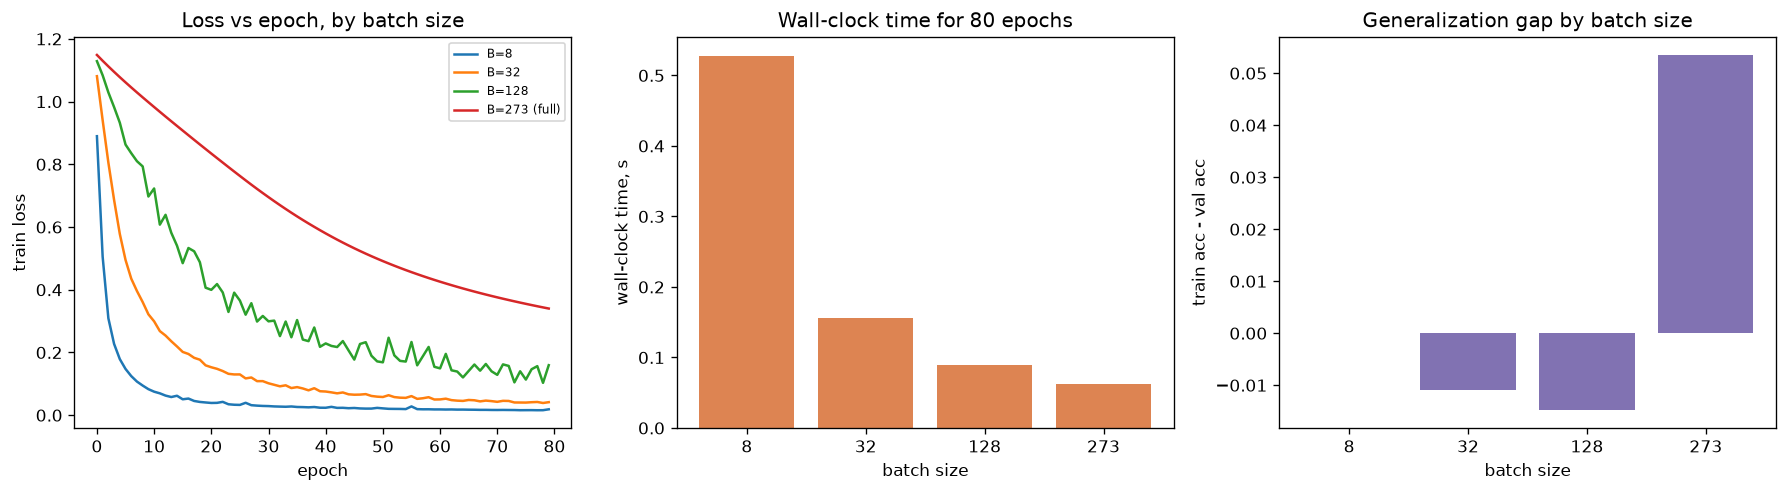
\includegraphics[width=0.95\textwidth]{figures/04_batch_size_sweep.png}
    \caption{Loss curves, wall-clock time, and generalization gap across the batch-size sweep.}
\end{figure}

\textbf{Smaller batches converge in far fewer epochs but cost more wall-clock time} --
B=8 took roughly 4x the wall-clock of full-batch for the identical 80-epoch run, because
Python-level dispatch overhead per mini-batch step dominates at this network's tiny
scale, even though B=8 reaches the loss target in a fifth of the epochs full-batch never
reaches it in. The generalization gap also tracks batch size cleanly: full-batch is the
only configuration with a \emph{positive} gap (training ahead of validation), consistent
with small-batch gradient noise acting as an implicit regulariser.

\subsection*{Learning rate scheduler vs fixed baseline}

\begin{figure}[H]
    \centering
    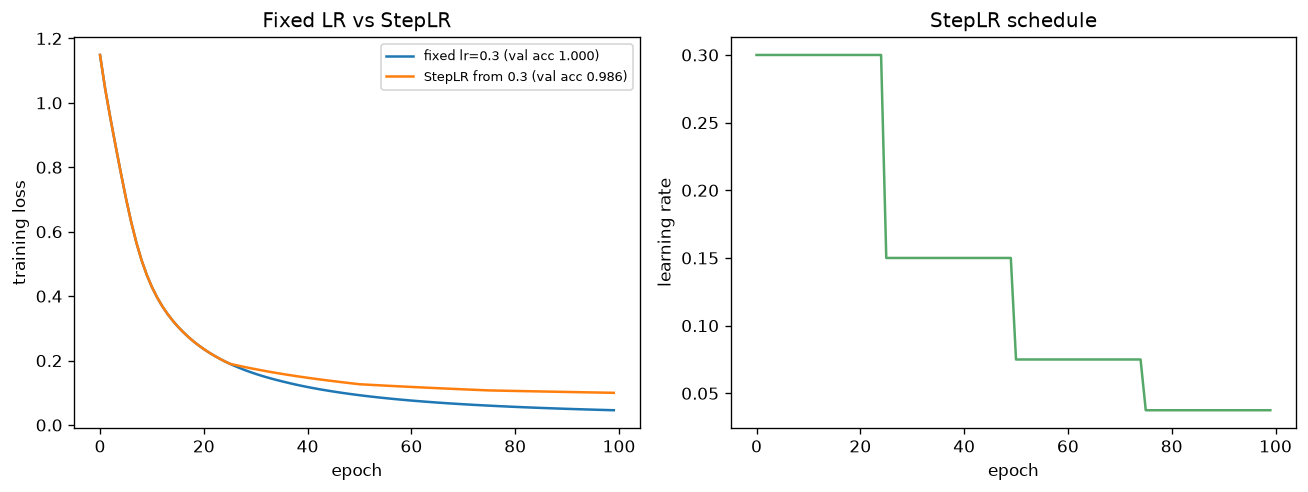
\includegraphics[width=0.95\textwidth]{figures/05_lr_scheduler.png}
    \caption{Fixed lr=0.3 (val acc 1.000) vs StepLR decaying from the same starting point (val acc 0.986).}
\end{figure}

\textbf{The schedule hurt here, not helped}: decaying an already-effective learning rate
just slowed further improvement, since there was no late-training instability for the
decay to fix. A schedule is a tool for a specific failure mode, not a free improvement,
and its value should be checked against a fixed-LR baseline rather than assumed.

\subsection*{Gradient accumulation, verified -- including the scaling bug}

\begin{table}[H]
\centering
\begin{tabular}{lr}
\toprule
\textbf{Accumulation method} & \textbf{Max diff vs direct large-batch gradient} \\
\midrule
Correctly scaled (loss $/ K$ before each backward) & $1.5\times10^{-8}$ (match) \\
Missing the $/K$ scaling & 4.00x too large \\
\bottomrule
\end{tabular}
\caption{$K=4$ micro-batches of 8, simulating one effective batch of 32.}
\end{table}

\subsection*{Gradient clipping, on a case built to explode}

\begin{figure}[H]
    \centering
    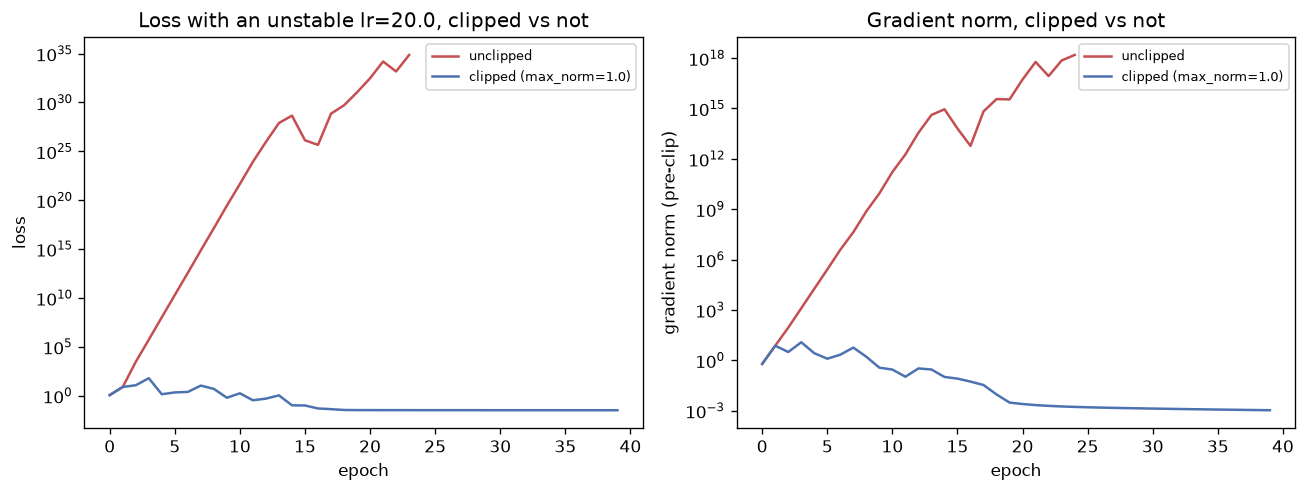
\includegraphics[width=0.95\textwidth]{figures/06_gradient_clipping.png}
    \caption{lr=20.0: unclipped loss diverges past $10^{35}$ by epoch 25; clipped (max\_norm=1.0) trains to a stable 0.033.}
\end{figure}

\subsection*{Early stopping, on a case built to overfit}

A 128-128-hidden network trained on a 20-row slice of the training data (deliberately
over-capacity for the data available).

\begin{figure}[H]
    \centering
    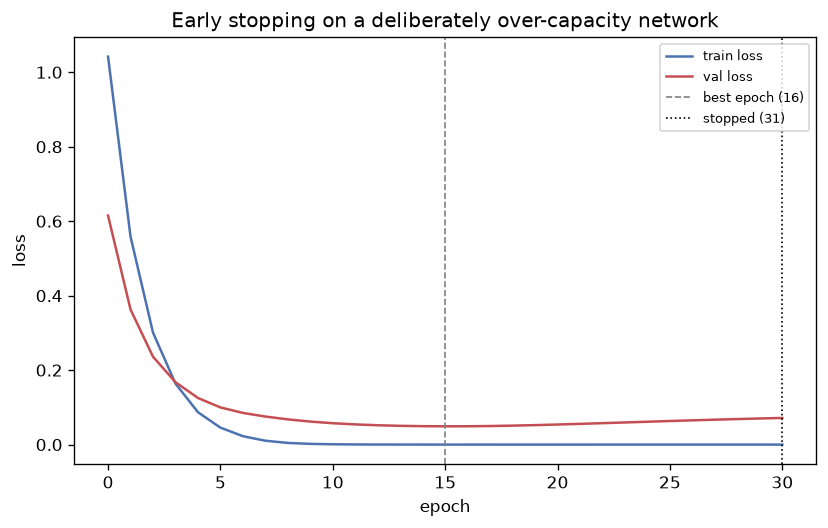
\includegraphics[width=0.68\textwidth]{figures/07_early_stopping.png}
    \caption{Train loss falls to 0; validation loss bottoms out at epoch 16 and rises afterward -- the overfitting signature.}
\end{figure}

Training stopped at epoch 31 of 300 planned (patience 15 after the best validation
epoch); restoring the epoch-16 weights rather than the final epoch's gave 97.1\%
validation accuracy.

% ----------------------------------------------------------------
\section*{Part D: Analysis \& Documentation}

\begin{table}[H]
\centering
\small
\begin{tabular}{lll}
\toprule
\textbf{Experiment} & \textbf{Configuration} & \textbf{Result} \\
\midrule
Optimizer verification & manual vs torch.optim & max diff $\le 5\times10^{-7}$, all three \\
Adam, uneven gradients & 1000x gradient-scale ratio & SGD stuck; Adam balanced on both axes \\
Optimizer comparison & SGD / SGD+mom / Adam & loss 0.093 / \textbf{0.012} / 0.033 \\
L2 vs weight decay & SGD / Adam & equivalent / NOT equivalent (0.067 diff) \\
Batch/mini-batch/SGD & B=273/32/1, same lr & loss 0.431 / 0.050 / 0.012 \\
Batch size sweep & B=8/32/128/273 & wall-clock 0.66/0.41/0.22/\textbf{0.16}s \\
LR schedule & fixed / StepLR & val acc \textbf{1.000} / 0.986 (schedule hurt) \\
Gradient accumulation & correct / missing $/K$ & match / 4.00x too large \\
Gradient clipping & unclipped / clipped & exploded to inf / stable, loss 0.033 \\
Early stopping & 128-128 net, 20-row subset & stopped epoch 31/300, val acc 0.971 \\
\bottomrule
\end{tabular}
\caption{Every experiment run in Parts B and C.}
\end{table}

\textbf{Best combination.} SGD with momentum (lr=0.1, momentum=0.9), batch size 32, no
learning-rate schedule. The 3-way optimizer comparison shows momentum reaching both the
lowest final loss and 100\% validation accuracy, ahead of plain SGD and Adam alike. The
batch-size sweep shows B=32 reaching 100\% validation accuracy in 11 epochs at less than
two-thirds of B=8's wall-clock cost for the same run -- B=8 is marginally faster in
epoch count but not in the metric that matters when training time is billed in
wall-clock seconds. The StepLR schedule made results worse, not better, so it is
excluded from the recommended configuration.

\textbf{Two counter-intuitive findings.}
\begin{enumerate}
    \item \emph{A larger batch size did not improve wall-clock convergence -- it was
    worse.} B=8 took $\sim$4x the wall-clock time of full-batch (B=273) for the
    identical 80-epoch budget, despite reaching the loss target in far fewer epochs.
    Small batches mean many more individual training steps per epoch, and per-step
    dispatch overhead (not the trivial arithmetic at this network's size) dominates
    wall-clock cost. Epoch count and wall-clock time measure genuinely different things
    and can disagree in either direction.
    \item \emph{Adam did not outperform tuned SGD+momentum} (final loss 0.0330 vs
    0.0123). Part B's worked example shows exactly the regime where Adam's adaptive
    scaling earns its keep: gradients differing by orders of magnitude across
    parameters. This small, well-conditioned network has no such pathology, so Adam's
    extra machinery buys nothing, and a well-tuned momentum term -- simpler, one fewer
    hyperparameter to get wrong -- wins outright.
\end{enumerate}

\textbf{A concrete implementation gotcha.} A mis-scaled gradient-accumulation loss --
constructed and measured directly above. Accumulating gradients over $K=4$ micro-batches
by calling \texttt{.backward()} on each micro-batch's already-averaged loss, without
first dividing that loss by $K$, produces a summed gradient exactly $K$ times larger
than the gradient a direct pass over the equivalent full batch would produce (measured:
4.00x). It was diagnosed the same way every optimizer in this report was trusted: never
assume an implementation is correct, verify it numerically against a ground truth (here,
the direct large-batch gradient) before training with it. The fix is one line -- divide
each micro-batch's loss by $K$ before \texttt{.backward()} -- so that $K$ summed
micro-gradients equal one averaged large-batch gradient.

\textbf{Conclusion.} The thread running through this task is the same one that ran
through Task 18: every claim was checked against an independent source rather than
taken from convention. Three optimizers were verified against \texttt{torch.optim}
step-for-step before being trusted for the real comparison; a hand-derived gradient was
checked against autograd; a gradient-accumulation implementation was checked against a
direct large-batch computation, and its failure mode was reproduced deliberately rather
than only described. What emerged was not "Adam is best" or "bigger batches are always
faster" -- the two most repeated defaults in casual practice -- but a specific,
evidenced recommendation (tuned SGD+momentum, batch size 32, no schedule) for this
network on this data, arrived at by measuring rather than assuming.

\vspace{0.4cm}
\noindent The notebook and README are on GitHub: {\small\scalebox{0.72}[1]{\url{https://github.com/AbdullahAmir06/ai-internship-abdullahamir}}}

\end{document}
